\chapter{Introduction}\label{ch:introduction}

\lipsum[3-5] 

\begin{figure}[ht]
    \begin{centering}
    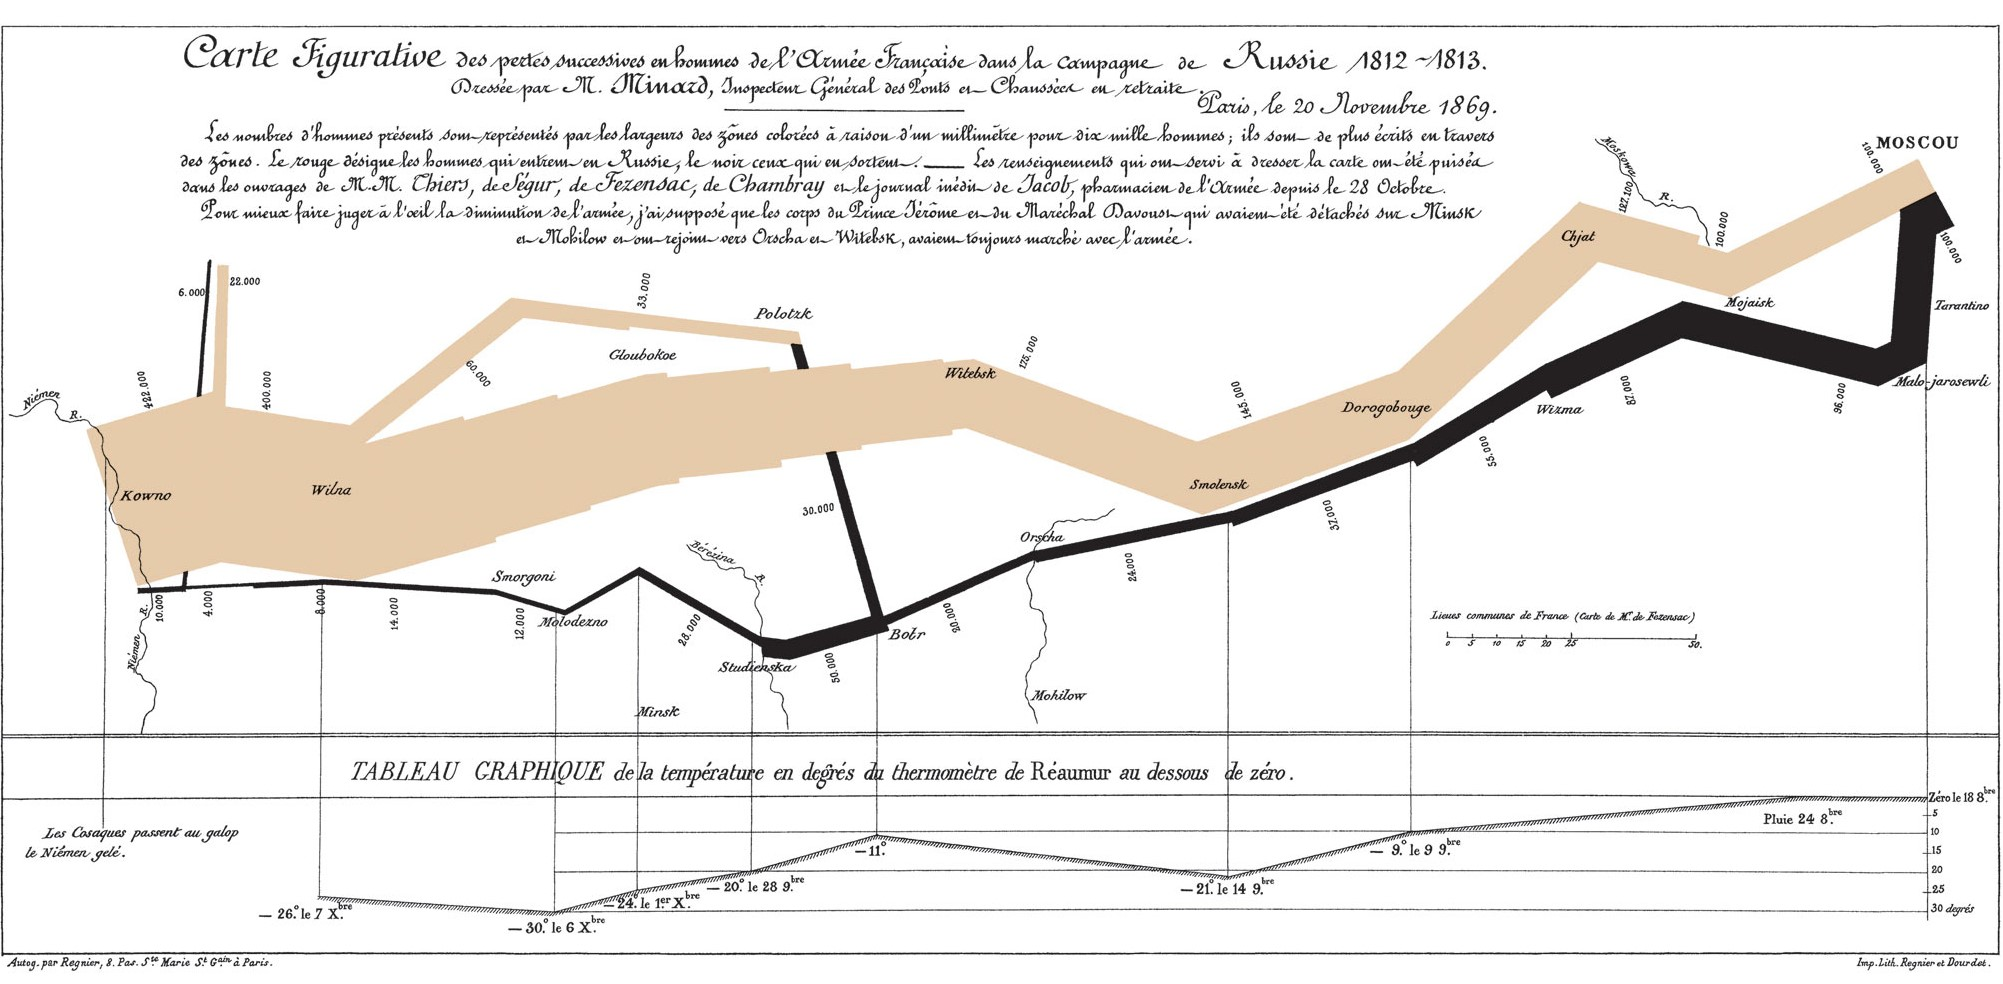
\includegraphics[width=0.8\linewidth]{figures/Minard.jpg}
    \par\end{centering}
    \caption[Napoleon's Invasion]{What may well be the greatest statistical graphic ever drawn~\cite{Tufte1983}\label{fig:MLP}}
\end{figure}

\section[More Lipsum]{Continuing on}\label{sec:lipsum}
\lipsum[6-10]~\cite{Min2023} \cref{fig:MLP}, \cref{tab:data}, \cref{eq:pn_taylor}, \cref{lst:listing-matlab}



\begin{table}[ht]
    \centering
    \small
    \begin{tabular}{SSSSSSSS} \toprule
        {\(m\)} & {\(\Re\{\underline{\mathfrak{X}}(m)\}\)} & {\(-\Im\{\underline{\mathfrak{X}}(m)\}\)} & {\(\mathfrak{X}(m)\)} & {\(\frac{\mathfrak{X}(m)}{23}\)} & {\(A_m\)} & {\(\varphi(m)\ /\ ^{\circ}\)} & {\(\varphi_m\ /\ ^{\circ}\)} \\ \midrule
        1  & 16.128 & +8.872 & 16.128 & 1.402 & 1.373 & -146.6 & -137.6 \\
        2  & 3.442  & -2.509 & 3.442  & 0.299 & 0.343 & 133.2  & 152.4  \\
        3  & 1.826  & -0.363 & 1.826  & 0.159 & 0.119 & 168.5  & -161.1 \\
        4  & 0.993  & -0.429 & 0.993  & 0.086 & 0.08  & 25.6   & 90     \\ \midrule
        5  & 1.29   & +0.099 & 1.29   & 0.112 & 0.097 & -175.6 & -114.7 \\
        6  & 0.483  & -0.183 & 0.483  & 0.042 & 0.063 & 22.3   & 122.5  \\
        7  & 0.766  & -0.475 & 0.766  & 0.067 & 0.039 & 141.6  & -122   \\
        8  & 0.624  & +0.365 & 0.624  & 0.054 & 0.04  & -35.7  & 90     \\ \midrule
        9  & 0.641  & -0.466 & 0.641  & 0.056 & 0.045 & 133.3  & -106.3 \\
        10 & 0.45   & +0.421 & 0.45   & 0.039 & 0.034 & -69.4  & 110.9  \\
        11 & 0.598  & -0.597 & 0.598  & 0.052 & 0.025 & 92.3   & -109.3 \\ \bottomrule
    \end{tabular}
    \caption[Random Data]{Table with random data.}\label{tab:data}
\end{table}

\begin{gather}
    V_{BE} = \frac{kT_0}{q} \Biggl\{ \ln{\biggl(\frac{I_C}{I_s T_0}\biggr)} + \Biggl[\ln{\biggl(\frac{I_C}{I_s T_0}\biggr)} - \biggl( \beta + \frac{E_{G_0}}{kT_0} \biggr) \Biggr] \biggl( \frac{T}{T_0} - 1 \biggr) \nonumber \\ - \frac{\beta}{2} {\biggl( \frac{T}{T_0} - 1 \biggr)}^2 + \cdots + \frac{\beta {(-1)}^{(n-1)}}{n(n-1)} {\biggl( \frac{T}{T_0} - 1 \biggr)}^n + \cdots \Biggr\}\label{eq:pn_taylor} \\
    V_{BE} > 4V_T,\qquad T < 2T_0 \nonumber
\end{gather}

\lstinputlisting[caption={[Matlab]Sample Code Listing Matlab}, label={lst:listing-matlab}, language=Matlab, style=Matlab-editor, basicstyle=\tiny]{code/code_sample.m}